\textbf{Name: } Patrick Harvey\\

\medskip

\textbf{Conspirators:} 

\medskip
\medskip

\hrule

\medskip


\begin{enumerate}

\item
  Derive Murray's law.

  Per lectures, find the minimum rate of energy expenditure
  working from the assertion that:
  \label{*}$$
  P
  =
  P_{\textnormal{drag}} + P_{\textnormal{met}}
  =
  \Phi^{2}
  \frac{
    8 \eta \ell
  }{
    \pi r^{4}
  }
  +
  c_{\textnormal{met}}
  r^{2}
  \ell,
  $$
  where met stands for metabolic.

  We are interested in how $P$ varies with the tube radius $r$.

  Per lectures, we defined the `parent' branch's radius as $r_{0}$,
  and the `offspring' branches as having radii $r_{1}$ and $r_{2}$
  (which need not be the same).

  Show that minimizing energy expenditure leads to
  $r_{0}^{3} = r_{1}^{3} + r_{2}^{3}$.

  Note that in the \LaTeX\ settings for assignments, various derivative notations
  are included.

  Here, you will want to use partial derivatives, and here's a start.

  Note the code-like formatting as expounded on
  \wordwikilink{https://pdodds.w3.uvm.edu/writings/2015-05-13better-writing-editing-thinking-with-line-breaks/}{here}.
  Far easier to create, edit, debug, read.

  \begin{LTXexample}
      $
    \partialdiff{P}{r}
    = 
    \partialdiff{}{r} 
    \left( 
    \Phi^{2}
    \frac{
      8 \eta \ell
    }{
      \pi r^{4}
    }
    +
    c_{\textnormal{met}}
    r^{2}
    \ell
    \right)
    $
  \end{LTXexample}
  
   \solutionstart

   See \ref{murray} for alternative derivation.
   
    Starting from:
    
    \begin{align*}
       \partialdiff{}{r} P
       &= 
       \partialdiff{}{r} 
       \left( 
       \Phi^{2}
       \frac{
            8 \eta \ell
       }{
            \pi r^{4}
       }
       +
       c_{\textnormal{met}}
       r^{2}
       \ell
       \right)
       \end{align*}
       We will let $\frac{8\eta}{\pi}=Z$
       
       \begin{align*}
       &= 
       \partialdiff{}{r} 
       \left(
       \Phi^{2}
       Z
       \left(
       r^{-4}
       \right)
       \ell
       +
       c_{\textnormal{met}}
       r^{2}
       \ell
       \right)
       \\
       &= 
       \partialdiff{}{r} 
       \left(
       \Phi^{2}
       Z
       \left(
       r^{-4}
       \right)
       \ell
       \right)
       +
       \partialdiff{}{r} 
       \left(
       c_{\textnormal{met}}
       r^{2}
       \ell
       \right)
       \\
       0 &= 
       \Phi^{2}
       Z
       \ell
       \left(
       -4
       (r^{-5})
       \right)
       +
       2 c_{\textnormal{met}} r
       \ell
       \\ 
       \Phi^{2}
       Z
       \ell
       \left(
       4 
       r^{ -5}
       \right)
       &=
       c_{\textnormal{met}}
       r
       \ell
       \\
       \Phi^{2}
       &=
       \frac{
       c_{\textnormal{met}}
       r
       \ell
       }
       {
       Z
       \ell
       \left(
       4
       r^{-5}
       \right)
       }
       \\
       &=
       \frac{
       c_{\textnormal{met}}
       \cancel{\ell}
       }
       {
       Z
       \cancel{\ell}
       }
       \frac{r}{
       \left(
       4 
       r^{-5}
       \right)}
       \\
       &=
       \frac{c_{\textnormal{met}}
       }{4 Z}
       \cdot
       r^{6}
       \end{align*}
    
       Here, we can consider the ratio of our constants
       $
       \frac{
       c_\textnormal{met}}
       {Z
       }
       $, and $1/4$ to be equal to a new constant $k^2$
       
       \begin{align*}
       \Phi^{2}
       &=
       \left(
       k^{2}
       \right)
       r^{6}
       \\
       \Phi
       &=
       \sqrt{
       k^{2}
       r^{6}
       }
       \\
       \Phi
       &=
       k
       r^3
       \\
       \Phi
       &\propto
       r^3
       \end{align*}
       
       With the relation $\Phi \propto r^3$ for (\ref{*}),
       and holding the forces in a steady state, we have:

       \begin{align*}
       \Phi_i  &=\Phi_{i+1} + \hdots + \Phi_j
       \\
       \textnormal{but for now...}
       \\
       r_0^3   &= r_1^3 + r_2^3
       \end{align*}
       \solutionend
    
    
    \item
      Derive the equivalent of Murray's law for branching
      networks where material moves by diffusion.
      Perhaps surprisingly, this connects
      the inner workings of insects,
      electrical networks, and search on networks.
    
      For diffusion,
      the impedance of a vessel is now
      $
      Z
      =
      c_{\textnormal{diff}}
      \ell
      r^{-2}
      $
      where
      $c_{\textnormal{diff}}$ is a constant,
      $\ell$ is vessel length,
      and $r$ is vessel radius.
    
      In terms of general impedance, the expression
      for the rate of energy expenditure is:
      $$
      P
      =
      P_{\textnormal{drag}} + P_{\textnormal{met}}
      =
      \Phi^{2}
      Z
      +
      c_{\textnormal{met}}
      r^{2} \ell.
      $$

  
   \solutionstart

   Starting from:

   \begin{align*}
   \partialdiff{}{r} P
   &= 
   \partialdiff{}{r} 
   \left( 
   \Phi^{2}
   \left(
   c_{\textnormal{diff}}
   \ell
   r^{-2}
   \right)
   +
   c_{\textnormal{met}}
   r^{2}
   \ell
   \right)
   \end{align*}
   
   We will proceed as before:
   
   \begin{align*}
   &= 
   \partialdiff{}{r}
   \left(
   \Phi^{2}
   c_{\textnormal{diff}}
   \ell
   r^{-2}
   \right)
   +
   \partialdiff{}{r}
   \left( 
   c_{\textnormal{met}}
   r^{2}
   \ell
   \right)
   \\
   &=
   \Phi^{2}
   c_{\textnormal{diff}}
   \ell
   \left(
   -2 
   r^{-3}
   \right)
   +
   2
   r
   c_{\textnormal{met}}
   \ell
   \\
   \Phi^{2}
   c_{\textnormal{diff}}
   \ell
   \left(
   2 
   r^{-3}
   \right)
   &=
   2
   r
   c_{\textnormal{met}}
   \ell
   \\
   \Phi^2
   &=
   \frac{
        c_{\textnormal{met}}
        \cancel{\ell}
        \left(
        \cancel{2}r
        \right)
   }{
        c_{\textnormal{diff}}
   \cancel{\ell}
   \left(
   \cancel{2} 
   r^{-3}
   \right)}
   \\
   \Phi
   &=
   \sqrt{k^2}
   \sqrt{r^4}\\
   &= kr^2
   \end{align*}
   
   With a function $\Phi$ of $r$, and maintaining the system in a steady state such that
   $\Phi_0 = \Phi_1 + \Phi_2$.

   \begin{align*}
   \cancel{k}
   r_0^{2}
   &=
   \cancel{k}
   r_1^{2}
   +
   \cancel{k}
   r_2^{2}
   \end{align*}

   Giving:

   \begin{equation}
   r_0^{2}
   &=
   r_1^{2}
   +
   r_2^{2}
   \label{eq:diff_deriv}
   \end{equation}

   Interestingly, we see that this relationship is the two-dimensional projection of the originally desired angular direction of a tubular structure sought by Murray, which might be handy for 5. 
   
   \solutionend

\item

  Now derive the generalized version of
  Murray's law for a generalized impedance
  $Z
  =
  c_{\textnormal{impedance}}
  \ell
  r^{-2\alpha}$,
  where
  $c_{\textnormal{imp}}$ is a
  general impedance constant,
  $\ell$ is vessel length,
  and $r$ is vessel radius.

  We can assume $\alpha > 0$ as impedance should decrease with wider vessels.

  We choose $r^{-2\alpha}$ because cross sectional area $\pi r^{2}$ can
  be considered the essential parameter here, and because we skipped to the end of the book
  and decided to rewrite the start.

  
   \solutionstart

   Picking up from \ref{*} and restructuring $r^{-4}$ such that $r^{-2 \cdot \alpha}$ if $\alpha = 2$

   \begin{align*}
   \partialdiff{}{r} P
   &= 
   \partialdiff{}{r} 
   \left( 
   \Phi^{2}
   \left(
   c_{\textnormal{imp}}
   \ell
   r^{-2\alpha}
   \right)
   +
   c_{\textnormal{met}}
   r^{2}
   \ell
   \right)
   \end{align*}
   
   We will proceed as before:
   
   \begin{align*}
   &= 
   \partialdiff{}{r}
   \left(
   \Phi^{2}
   c_{\textnormal{imp}}
   \ell
   r^{-2\alpha}
   \right)
   +
   \partialdiff{}{r}
   \left( 
   c_{\textnormal{met}}
   r^{2}
   \ell
   \right)
   \\
   &=
   \Phi^{2}
   c_{\textnormal{imp}}
   \ell
   \left(
   -2\alpha 
   r^{-2\alpha-1}
   \right)
   +
   2
   r
   c_{\textnormal{met}}
   \ell
   \\
   \Phi^{2}
   c_{\textnormal{imp}}
   \ell
   \left(
   2 \alpha 
   r^{-2\alpha-1}
   \right)
   &=
   2
   r
   c_{\textnormal{met}}
   \ell
   \\
   \Phi^2
   &=
   \frac{
        c_{\textnormal{met}}
        \cancel{\ell}
        \left(
        \cancel{2}r
        \right)
   }{
        c_{\textnormal{imp}}
   \cancel{\ell}
   \left(
   \cancel{2}
   \alpha 
   r^{-2\alpha-1}
   \right)}
   \\
   \Phi
   &=
   \sqrt{k^2}
   \sqrt{\frac{r}{\alpha 
   r^{-2\alpha-1}}}\\
   &= k (r^{\alpha+1}) \alpha^{-1/2}
   \end{align*}

   Giving a representation for $\Phi$ proportional to:
   \begin{equation}
   \Phi
   &\propto
   (r^{\alpha+1}) \alpha^{-1/2}
   \label{eq:imp_phi}
   \end{equation}

   With a function $\Phi$ of $r$, we want a closed system in a steady state such that $
   \Phi_0 = \Phi_1 + \Phi_2$.

   \begin{align*}
   \cancel{\alpha^{-1/2}
   k}
   r_0^{1+\alpha}
   &=
   \cancel{\alpha^{-1/2}
   k}
   r_1^{1+\alpha}
   +
   \cancel{\alpha^{-1/2}
   k}
   r_2^{1+\alpha}
   \end{align*}

   Recalling $\alpha = 2$ we have a unit relationship of:

   \begin{equation}
   r_0^{3} \frac{1}{\sqrt[3]{2}}
   &=
   r_1^{3} \frac{1}{\sqrt[3]{2}}
   +
   r_2^{3} \frac{1}{\sqrt[3]{2}}
   \label{eq:murray_deriv}
   \end{equation}
   Leading to interesting interpretations for Murray and a function $\Phi$ of $r$, for a closed system in a steady state such that $
   \Phi_i = \Phi_{i+1} + \hdots + \Phi_{j}$ gives:

   \begin{align*}
   \pi \frac{r_i^{\alpha+1}}{\sqrt[\alpha+1]{2}}
   &=
   \pi \frac{r_{i+1}^{\alpha+1}}{\sqrt[\alpha+1]{2}}
   +
   \hdots
   +
   \pi \frac{r_{j}^{\alpha+1}}{\sqrt[\alpha+1]{2}}\\
   \end{align*}
   \clearpage

   
   $\textbf{Murray's derivation:}$
   \\
   \label{murray}\\
   \\Murray's conceptual framework for the optimal transport of a Newtonian fluid through a tubular structure relied on an assumption that the following equation holds:
   \begin{equation}
   E
   =
   pf
   +
   bvol
   =
   \frac{
   f^2
   \cdot l
   \cdot 8 \eta
   }{
   \pi
   r^4
   }
   +
   bl\pi
   r^2
   \label{eq:P}
   \end{equation}
   
   Where $p =$ loss of pressure; $f^2=$ constant flow rate; $b =$ basal energy (ergs/cc. sec.); $vol =$ volume; $l =$ length of tubular body; $r =$ radius; and $\eta =$ viscosity.

   Murray holds the length ($l$) constant, to arrive at the following equation for \textit{any} steady state of the system. That is, for constant flow rate $f^2$ (or $\Phi^2$) and fixed length $l$, we have:

   \begin{equation}
   f^2
   =
   \frac{
   r^6
   \pi^2
   b
   }
   {
   16\eta
   }
   \label{eq:murrays_sol}
   \end{equation}

   substituting $f^2$ into (\ref{eq:P}) to get:

   \begin{equation}
   E/l = r^2 (3 \pi b)
   \label{eq:E_l}
   \end{equation}
   
   and consolidating constants to $k$ for:
   
   \begin{equation}
   (kE)/l = r^2
   \label{eq:r**2}
   \end{equation}

   This method claims that $r^2 \propto E/l$ (or if we are feeling fiendish $\pi r^2 = E \frac{\pi}{l}$) and fixes the radii of children branches to their angle of departure from the parent branch (giving Murray's law $r_0^3 = r_1^3 + r_2^3$ the optimal angular direction for $n$ branches of a single source).

   Murray considers three cases of "Y" shaped bifurcations, as well as a special case where a bifurcation of equal sized children is joined with a continuation of the parent branch along the same trajectory, but with a reduced radius in order to maintain a steady state. The illustration below gives an example of Murray's conceptual framework:
   
   \begin{center}
   \includegraphics[width=0.85\textwidth]{figures/56246342-CF31-4755-AE77-2135BDF0DADE.jpeg}
   \end{center}

   \solutionend

\item
  Murray's law for real data.

  See if you can track down a data set for real branching networks
  where Murray's law might reasonably apply, and then test how
  well Murray's law holds up.

  Could be blood vessels, trees, \ldots~\cite{sherman1981a,mcculloh2003a,mcculloh2004a}.

  As always, you are welcome to collaborate.
  Feel free to share data sets on Teams.

  
   \solutionstart

   Interesting to reconsider forest fire model with balancing force of forest regrowth as a weighted projection on the lattice. \url{https://www.fs.usda.gov/rds/archive/products/RDS-2020-0079/RDS-2020-0079.zip}

   \solutionend

  


\item (3 + 3)

  Let's start on trying to reproduce
  reproduce Bohn and Magnasco's Figs.~2a and 2b in~\cite{bohn2007a}.

  A profound physical result. For movement of stuff, when should networks exist?

  Preliminary work:

  \begin{itemize}
  \item 
    Construct an adjacency matrix for
    the underlying hexagonal lattice where
    the side number of nodes is a variable $n$.
  \item
    Plot the $n=8$ version to match with the
    grids underlying the figures below.
  \end{itemize}

  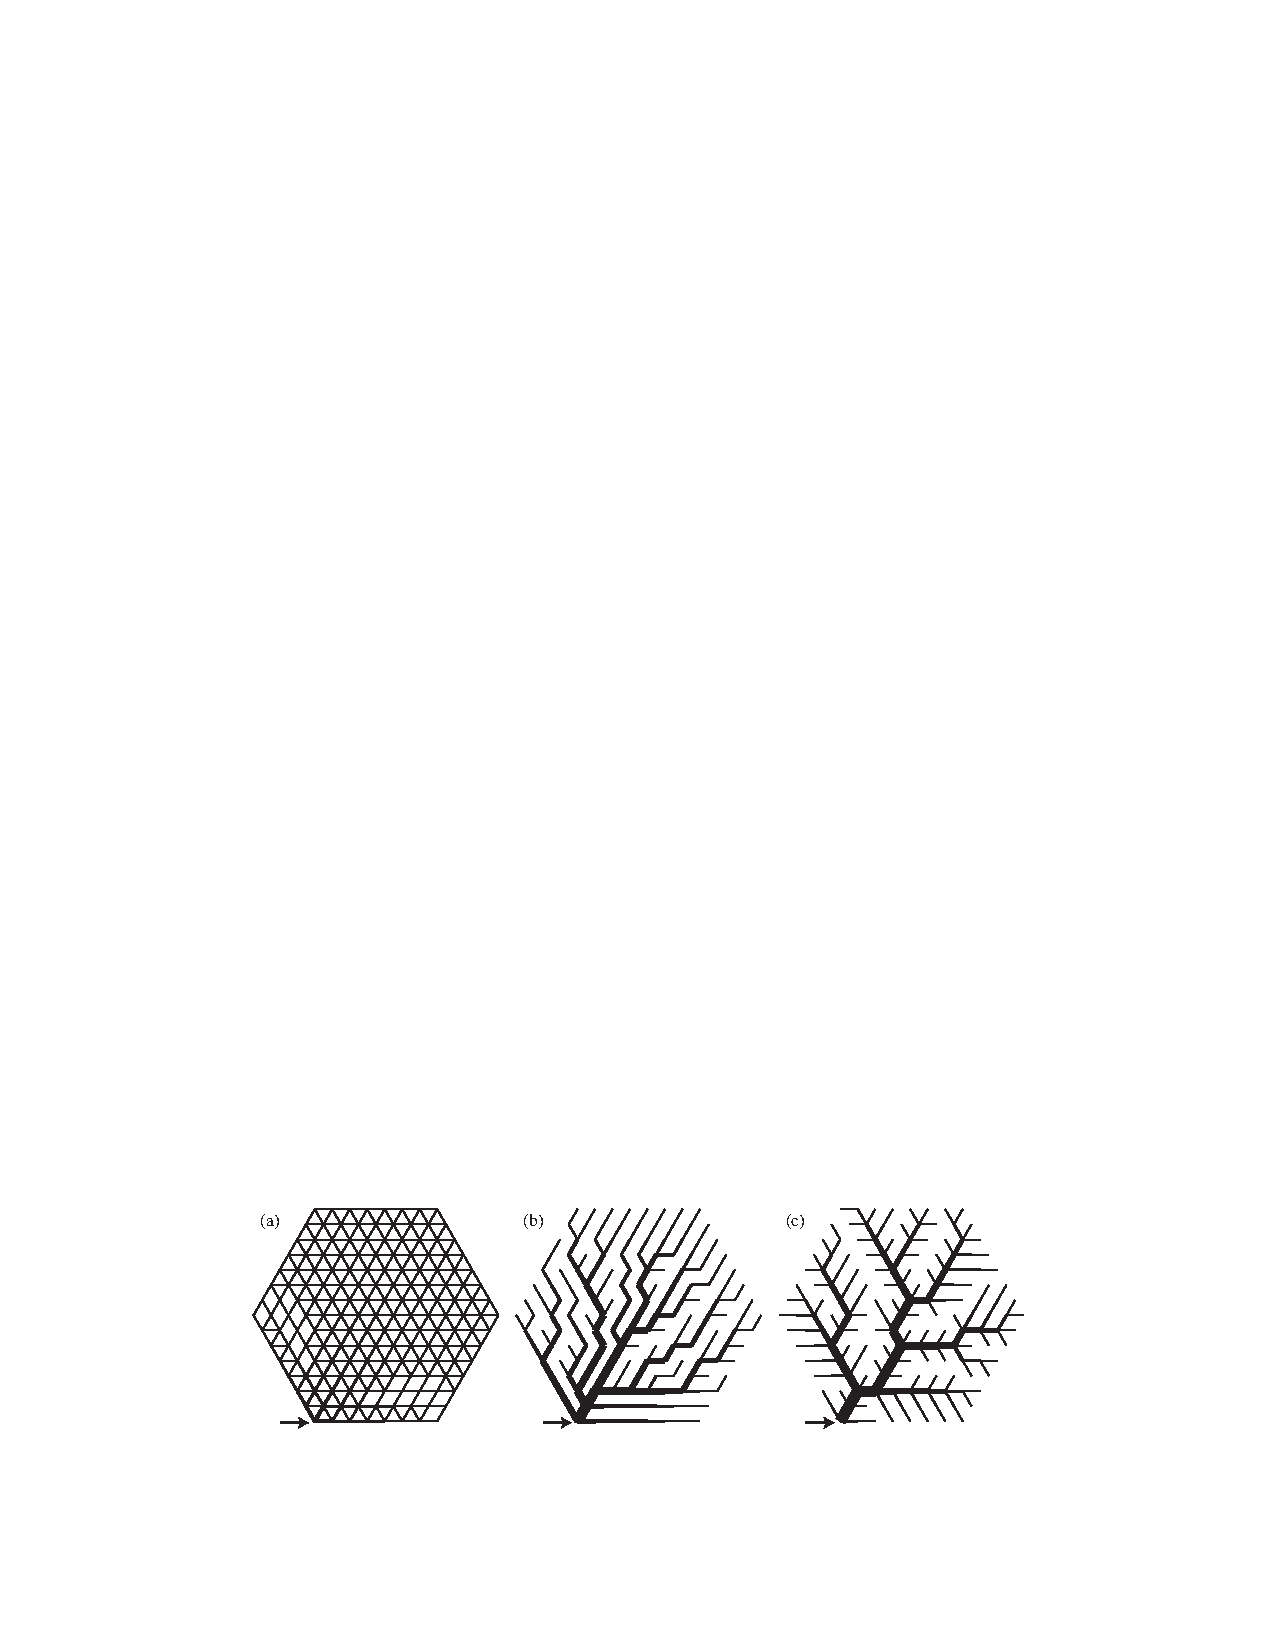
\includegraphics[width=\textwidth]{bohn2007a_fig2.pdf}


  
\end{enumerate}